%% This file was auto-generated by IPython.
%% Conversion from the original notebook file:
%% pcaperf.ipynb
%%
\documentclass[11pt,english,fleqn]{article}

%% This is the automatic preamble used by IPython.  Note that it does *not*
%% include a documentclass declaration, that is added at runtime to the overall
%% document.

\usepackage{amsmath}
\usepackage{amssymb}
\usepackage{graphicx}
\usepackage{ucs}
\usepackage[utf8x]{inputenc}

% needed for markdown enumerations to work
\usepackage{enumerate}

% Slightly bigger margins than the latex defaults
\usepackage{geometry}
\geometry{verbose,tmargin=3cm,bmargin=3cm,lmargin=2.5cm,rmargin=2.5cm}

% Define a few colors for use in code, links and cell shading
\usepackage{color}
\definecolor{orange}{cmyk}{0,0.4,0.8,0.2}
\definecolor{darkorange}{rgb}{.71,0.21,0.01}
\definecolor{darkgreen}{rgb}{.12,.54,.11}
\definecolor{myteal}{rgb}{.26, .44, .56}
\definecolor{gray}{gray}{0.45}
\definecolor{lightgray}{gray}{.95}
\definecolor{mediumgray}{gray}{.8}
\definecolor{inputbackground}{rgb}{.95, .95, .85}
\definecolor{outputbackground}{rgb}{.95, .95, .95}
\definecolor{traceback}{rgb}{1, .95, .95}

% Framed environments for code cells (inputs, outputs, errors, ...).  The
% various uses of \unskip (or not) at the end were fine-tuned by hand, so don't
% randomly change them unless you're sure of the effect it will have.
\usepackage{framed}

% remove extraneous vertical space in boxes
\setlength\fboxsep{0pt}

% codecell is the whole input+output set of blocks that a Code cell can
% generate.

% TODO: unfortunately, it seems that using a framed codecell environment breaks
% the ability of the frames inside of it to be broken across pages.  This
% causes at least the problem of having lots of empty space at the bottom of
% pages as new frames are moved to the next page, and if a single frame is too
% long to fit on a page, will completely stop latex from compiling the
% document.  So unless we figure out a solution to this, we'll have to instead
% leave the codecell env. as empty.  I'm keeping the original codecell
% definition here (a thin vertical bar) for reference, in case we find a
% solution to the page break issue.

%% \newenvironment{codecell}{%
%%     \def\FrameCommand{\color{mediumgray} \vrule width 1pt \hspace{5pt}}%
%%    \MakeFramed{\vspace{-0.5em}}}
%%  {\unskip\endMakeFramed}

% For now, make this a no-op...
\newenvironment{codecell}{}

 \newenvironment{codeinput}{%
   \def\FrameCommand{\colorbox{inputbackground}}%
   \MakeFramed{\advance\hsize-\width \FrameRestore}}
 {\unskip\endMakeFramed}

\newenvironment{codeoutput}{%
   \def\FrameCommand{\colorbox{outputbackground}}%
   \vspace{-1.4em}
   \MakeFramed{\advance\hsize-\width \FrameRestore}}
 {\unskip\medskip\endMakeFramed}

\newenvironment{traceback}{%
   \def\FrameCommand{\colorbox{traceback}}%
   \MakeFramed{\advance\hsize-\width \FrameRestore}}
 {\endMakeFramed}

% Use and configure listings package for nicely formatted code
\usepackage{listingsutf8}
\lstset{
  language=python,
  inputencoding=utf8x,
  extendedchars=\true,
  aboveskip=\smallskipamount,
  belowskip=\smallskipamount,
  xleftmargin=2mm,
  breaklines=true,
  basicstyle=\small \ttfamily,
  showstringspaces=false,
  keywordstyle=\color{blue}\bfseries,
  commentstyle=\color{myteal},
  stringstyle=\color{darkgreen},
  identifierstyle=\color{darkorange},
  columns=fullflexible,  % tighter character kerning, like verb
}

% The hyperref package gives us a pdf with properly built
% internal navigation ('pdf bookmarks' for the table of contents,
% internal cross-reference links, web links for URLs, etc.)
\usepackage{hyperref}
\hypersetup{
  breaklinks=true,  % so long urls are correctly broken across lines
  colorlinks=true,
  urlcolor=blue,
  linkcolor=darkorange,
  citecolor=darkgreen,
  }

% hardcode size of all verbatim environments to be a bit smaller
\makeatletter 
\g@addto@macro\@verbatim\small\topsep=0.5em\partopsep=0pt
\makeatother 

% Prevent overflowing lines due to urls and other hard-to-break entities.
\sloppy

\setlength{\mathindent}{0pt}
\setlength{\parindent}{0pt}
\setlength{\parskip}{8pt}
\begin{document}

SVD ile PCA Hesaplamak

PCA bolumunde anlatilan yontem temel bilesenlerin hesabinda ozdegerler
ve ozvektorler kullandi. Alternatif bir yontem Tekil Deger Ayristirma
(Singular Value Decomposition -SVD-) uzerinden bu hesabi yapmaktir. SVD
icin Lineer Cebir Ders 29'a bakabilirsiniz. Peki ne zaman klasik PCA ne
zaman SVD uzerinden PCA kullanmali? Bir cevap belki mevcut
kutuphanelerde SVD kodlamasinin daha iyi olmasi, ayristirmanin ozvektor
/ deger hesabindan daha hizli isleyebilmesi {[}6{]}.

Ayrica birazdan gorecegimiz gibi SVD, kovaryans matrisi uzerinde degil,
$A$'nin kendisi uzerinde isletilir, bu hem kovaryans hesaplama asamasini
atlamamizi, hem de kovaryans hesabi sirasinda ortaya cikabilecek numerik
puruzlerden korunmamizi saglar (cok ufak degerlerin kovaryans hesabini
bozabilecegi literaturde bahsedilmektedir).

PCA ve SVD baglantisina gelelim:

Biliyoruz ki SVD bir matrisi su sekilde ayristirir
\[A = USV^T\]
$U$ matrisi $n \times n$ dikgen (orthogonal), $V$ ise $m \times m$
dikgen. $S$'in sadece kosegeni uzerinde degerler var ve bu $\sigma_j$
degerleri $A$'nin tekil degerleri (singular values) olarak biliniyor.

Simdi $A$ yerine $AA^T$ koyalim, yani $A$'nin kovaryans matrisinin SVD
ayristirmasini yapalim, acaba elimize ne gececek?
\[ AA^T = (USV^T)(USV^T)^T \]\[ = (USV^T)(V S^T U^T) \]\[ = U S S^T U^T \]
$S$ bir kosegen matrisi, o zaman $SS^T$ matrisi de kosegen, tek farkla
kosegen uzerinde artik $\sigma_j^2$ degerleri var. Bu normal.

$SS^T$ yerine $\Lambda$ sembolunu kullanalim, ve denklemi iki taraftan
(ve sagdan) $U$ ile carparsak (unutmayalim $U$ ortanormal bir matris ve
$U^T U = I$),
\[ AA^TU = U \Lambda U^TU \]\[ AA^TU = U \Lambda   \]
Son ifadeye yakindan bakalim, $U$'nun tek bir kolonuna, $u_k$ diyelim,
odaklanacak olursak, ustteki ifadeden bu sadece kolona yonelik nasil bir
esitlik cikartabilirdik? Soyle cikartabilirdik,
\[ (AA^T)u_k = \sigma^2 u_k   \]
Bu ifade tanidik geliyor mu? Ozdeger / ozvektor klasik yapisina eristik.
Ustteki esitlik sadece ve sadece eger $u_k$, $AA^T$'nin ozvektoru ve
$\sigma^2$ onun ozdegeri ise gecerlidir. Bu esitligi tum $U$ kolonlari
icin uygulayabilecegimize gore demek ki $U$'nun kolonlarinda $AA^T$'nin
ozvektorleri vardir, ve $AA^T$'nin ozdegerleri $A$'nin tekil
degerlerinin karesidir.

Bu muthis bir bulus. Demek ki $AA^T$'nin ozektorlerini hesaplamak icin
$A$ uzerinde SVD uygulayarak $U$'yu bulmamiz yeterli, kovaryans
matrisini hesaplamak bile gerekmiyor! $AA^T$ ozdegerleri uzerinde
buyukluk karsilastirmasi icin ise $A$'nin tekil degerlerine bakmak
yeterli!

Ornek

Ilk PCA yazisindaki ornege donelim, ve ozvektorleri SVD uzerinden
hesaplatalim. Once eig usulu ile

\begin{codecell}
\begin{codeinput}
\begin{lstlisting}
from pandas import *
data = read_csv("testSet.txt",sep="\t",header=None)
means = mean(data, axis=0)
meanless_data = data - means
cov_mat = cov(meanless_data, rowvar=0)
eigs,eigv = linalg.eig(mat(cov_mat))
eigv
\end{lstlisting}
\end{codeinput}
\begin{codeoutput}
\begin{verbatim}
matrix([[-0.85389096, -0.52045195],
        [ 0.52045195, -0.85389096]])
\end{verbatim}
\end{codeoutput}
\end{codecell}
Simdi de SVD usulu ile

\begin{codecell}
\begin{codeinput}
\begin{lstlisting}
U,s,Vt = svd(meanless_data.T,full_matrices=False)
U

\end{lstlisting}
\end{codeinput}
\begin{codeoutput}
\begin{verbatim}
array([[-0.52045195, -0.85389096],
       [-0.85389096,  0.52045195]])
\end{verbatim}
\end{codeoutput}
\end{codecell}
\begin{codecell}
\begin{codeinput}
\begin{lstlisting}
np.dot(U.T,U)
\end{lstlisting}
\end{codeinput}
\begin{codeoutput}
\begin{verbatim}
array([[ 1.,  0.],
       [ 0.,  1.]])
\end{verbatim}
\end{codeoutput}
\end{codecell}
Goruldugu gibi ayni ozvektorleri bulduk.

New York Times Yazıları Analizi
Simdi daha ilginc bir ornege bakalim. Bir arastirmaci belli yillar
arasindaki NY Times makalelerinde her yazida hangi kelimenin kac kere
ciktiginin verisini toplamis {[}1,2,3{]}, bu veri 4000 kusur kelime, her
satir (yazi) icin bir boyut (kolon) olarak kaydedilmis. Bu veri
nytimes.csv uzerinde ek bir normalize isleminden sonra, onun uzerinde
boyut indirgeme yapabiliriz.

Veri setinde her yazi ayrica ek olarak sanat (arts) ve muzik (music)
olarak etiketlenmis, ama biz PCA kullanarak bu etiketlere hic bakmadan,
verinin boyutlarini azaltarak acaba verinin ``ayrilabilir'' hale
indirgenip indirgenemedigine bakacagiz. Sonra etiketleri veri ustune
koyup sonucun dogrulugunu kontrol edecegiz.

Bakmak derken veriyi (en onemli) iki boyuta indirgeyip sonucu
grafikleyecegiz. Illa 2 olmasi gerekmez tabii, 10 boyuta indirgeyip (ki
4000 kusur boyuttan sonra bu hala muthis bir kazanim) geri kalanlar
uzerinde mesela bir kumeleme algoritmasi kullanabilirdik.

Ana veriyi yukleyip birkac satirini ve kolonlarini gosterelim.

\begin{codecell}
\begin{codeinput}
\begin{lstlisting}
from pandas import *
import numpy.linalg as lin
nyt = read_csv ("nytimes.csv")
labels = nyt['class.labels']
nyt.ix[:8,102:107]
\end{lstlisting}
\end{codeinput}
\begin{codeoutput}
\begin{verbatim}
   after  afternoon  afterward  again  against
0      1          0          0      0        0
1      1          1          0      0        0
2      1          0          0      1        2
3      3          0          0      0        0
4      0          1          0      0        0
5      0          0          0      1        2
6      7          0          0      0        1
7      0          0          0      0        0
8      0          0          0      0        0
\end{verbatim}
\end{codeoutput}
\end{codecell}
Yuklemeyi yapip sadece etiketleri aldik ve onlari bir kenara koyduk.
Simdi onemli bir normalizasyon islemi gerekiyor - ki bu isleme ters
dokuman-frekans agirliklandirmasi (inverse document-frequency weighting
-IDF-) ismi veriliyor - her dokumanda aşırı fazla ortaya cikan
kelimelerin onemi ozellikle azaltiliyor, ki diger kelimelerin etkisi
artabilsin.

IDF kodlamasi alttaki gibidir. Once class.labels kolonunu atariz. Sonra
``herhangi bir deger iceren'' her hucrenin 1 digerlerinin 0 olmasi icin
kullanilan DataFrame uzerinde astype(bools) isletme numarasini
kullaniriz, boylece asiri buyuk degerler bile sadece 1 olacaktir. Bazi
diger islemler sonrasi her satiri kendi icinde tekrar normalize etmek
icin o satirdaki tum degerlerin karesinin toplaminin karekokunu aliriz
ve satirdaki tum degerler bu karekok ile bolunur. Buna oklitsel
(euclidian) normalizasyon denebilir.

Not: Oklitsel norm alirken toplamin hemen ardindan cok ufak bir 1e-16
degeri eklememize dikkat cekelim, bunu toplamin sifir olma durumu icin
yapiyoruz, ki sonra sifirla bolerken NaN sonucundan kacinalim.

\begin{codecell}
\begin{codeinput}
\begin{lstlisting}
nyt = nyt.drop(['class.labels'],axis=1)
freq = nyt.astype(bool).sum(axis=0)
freq = freq.replace(0,1)
w = np.log(float(nyt.shape[0])/freq)
nyt = nyt.apply(lambda x: x*w,axis=1)
nyt = nyt.apply(lambda x: x / np.sqrt(np.sum(np.square(x))+1e-16), axis=1)

\end{lstlisting}
\end{codeinput}
\end{codecell}
\begin{codecell}
\begin{codeinput}
\begin{lstlisting}
nyt=nyt.ix[:,1:] # ilk kolonu atladik
nyt.ix[:8,102:107]
\end{lstlisting}
\end{codeinput}
\begin{codeoutput}
\begin{verbatim}
   afterward     again   against       age  agent
0          0  0.000000  0.000000  0.051085      0
1          0  0.000000  0.000000  0.000000      0
2          0  0.021393  0.045869  0.000000      0
3          0  0.000000  0.000000  0.000000      0
4          0  0.000000  0.000000  0.000000      0
5          0  0.024476  0.052480  0.000000      0
6          0  0.000000  0.008536  0.000000      0
7          0  0.000000  0.000000  0.000000      0
8          0  0.000000  0.000000  0.000000      0
\end{verbatim}
\end{codeoutput}
\end{codecell}
SVD yapalim

\begin{codecell}
\begin{codeinput}
\begin{lstlisting}
nyt = nyt - nyt.mean(0)
u,s,v = lin.svd(nyt.T,full_matrices=False)
\end{lstlisting}
\end{codeinput}
\end{codecell}
\begin{codecell}
\begin{codeinput}
\begin{lstlisting}
s[:10]
\end{lstlisting}
\end{codeinput}
\begin{codeoutput}
\begin{verbatim}
array([ 1.41676764,  1.37161893,  1.31840061,  1.24567955,  1.20596873,
        1.18624932,  1.15118771,  1.13820504,  1.1138296 ,  1.10424634])
\end{verbatim}
\end{codeoutput}
\end{codecell}
\begin{codecell}
\begin{codeinput}
\begin{lstlisting}
u.shape
\end{lstlisting}
\end{codeinput}
\begin{codeoutput}
\begin{verbatim}
(4430, 102)
\end{verbatim}
\end{codeoutput}
\end{codecell}
SVD'nin verdigi $u$ icinden iki ozvektoru seciyoruz (en bastakiler,
cunku Numpy SVD kodu bu ozvektorleri zaten siralanmis halde dondurur),
ve veriyi bu yeni kordinata izdusumluyoruz.

\begin{codecell}
\begin{codeinput}
\begin{lstlisting}
proj = np.dot(nyt, u[:,:2])
proj.shape
plot(proj[:,0],proj[:,1],'.')

\end{lstlisting}
\end{codeinput}
\begin{codeoutput}
\begin{verbatim}
[<matplotlib.lines.Line2D at 0xb03bb2c>]
\end{verbatim}
\begin{center}
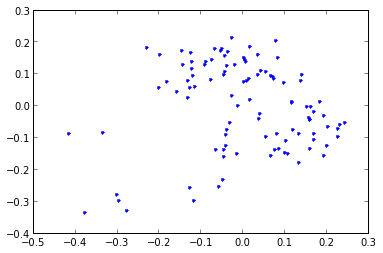
\includegraphics[width=0.7\textwidth]{pcaperf_files/pcaperf_fig_00.png}
\par
\end{center}
\end{codeoutput}
\end{codecell}
Simdi ayni veriyi bir de etiket bilgisini devreye sokarak cizdirelim.
Sanat kirmizi muzik mavi olacak.

\begin{codecell}
\begin{codeinput}
\begin{lstlisting}
arts =proj[labels == 'art']
music =proj[labels == 'music']
plot(arts[:,0],arts[:,1],'r.')
plot(music[:,0],music[:,1],'b.')
\end{lstlisting}
\end{codeinput}
\begin{codeoutput}
\begin{verbatim}
[<matplotlib.lines.Line2D at 0xb58eecc>]
\end{verbatim}
\begin{center}
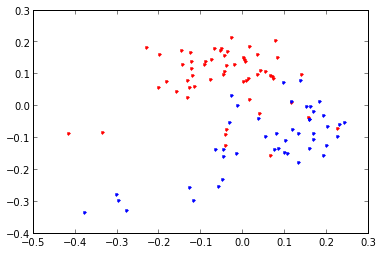
\includegraphics[width=0.7\textwidth]{pcaperf_files/pcaperf_fig_01.png}
\par
\end{center}
\end{codeoutput}
\end{codecell}
Goruldugu gibi veride ortaya cikan / ozvektorlerin kesfettigi dogal
ayirim, hakikaten dogruymus.

Metotun ne yaptigina dikkat, bir suru boyutu bir kenara atmamiza ragmen
geri kalan en onemli 2 boyut uzerinden net bir ayirim ortaya
cikartabiliyoruz. Bu PCA yonteminin iyi bir is becerdigini gosteriyor,
ve kelime sayilarinin makalelerin icerigi hakkinda ipucu icerdigini
ispatliyor.

{[}1{]} Cosma Rohilla Shalizi, Advanced Data Analysis from an Elementary
Point of View

{[}2{]}
http://www.ldc.upenn.edu/Catalog/CatalogEntry.jsp?catalogId=LDC2008T19

{[}3{]} http://www.stat.cmu.edu/\ensuremath{\sim}cshalizi/490/pca/

{[}5{]}
http://www.math.nyu.edu/faculty/goodman/teaching/RPME/notes/Section3.pdf

{[}6{]} Lineer Cebir notlarimizda SVD turetilmesine bakinca
ozdeger/vektor mantigina atif yapildigini gorebiliriz ve akla su
gelebilir; ``ozdeger / vektor rutini isletmekten kurtulalim dedik, SVD
yapiyoruz, ama onun icinde de ozdeger/vektor hesabi var''. Fakat sunu
belirtmek gerekir ki SVD numerik hesabini yapmanin tek yontemi
ozdeger/vektor yontemi degildir. Mesela Numpy Linalg kutuphanesi
icindeki SVD, LAPACK dgesdd rutinini kullanir ve bu rutin ic
kodlamasinda QR, ve bir tur bol / istila et (divide and conquer)
algoritmasi isletmektedir.

\end{document}
